%&tex
\documentclass{standalone}

\usepackage[dvipsnames]{xcolor}

\usepackage{tikz}
\usetikzlibrary{positioning}

\begin{document}

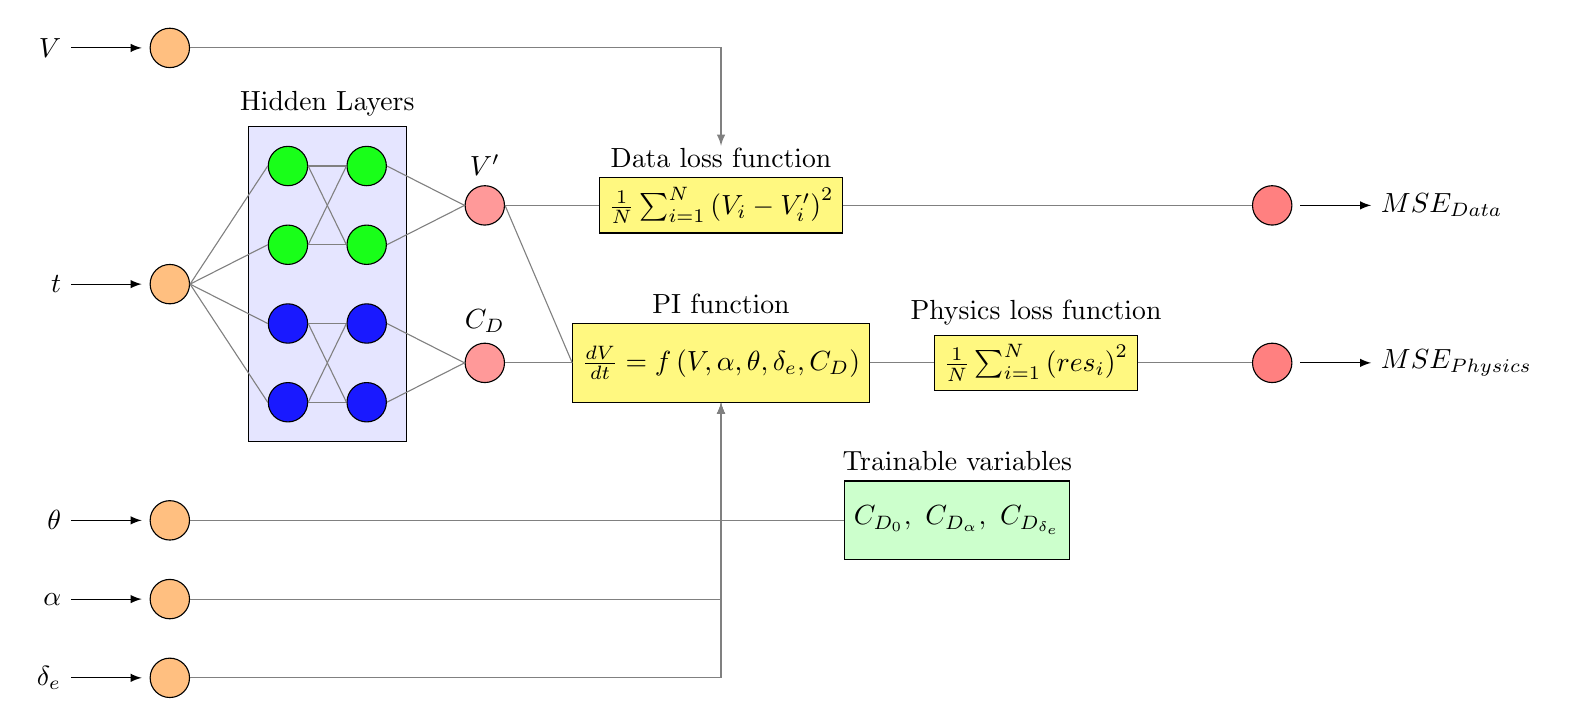
\begin{tikzpicture}
    % input layer node
    \node[draw,
    circle,
    minimum size = 0.5cm,
    fill=orange!50] (Time) at (0,0) {};

    % secondary input nodes
    \node[draw,
    circle,
    minimum size = 0.5 cm,
    fill=orange!50] (theta) at (0,-3){};
    \node[draw,
    circle,
    minimum size = 0.5 cm,
    fill=orange!50] (alpha) at (0,-4){};
    \node[draw,
    circle,
    minimum size = 0.5 cm,
    fill=orange!50] (dele) at (0,-5){};
    \node[draw,
    circle,
    minimum size = 0.5 cm,
    fill=orange!50] (V_inp) at (0,3){};

    % hidden layer cover
    \node[draw,
    rectangle,
    minimum width = 2 cm,
    minimum height = 4 cm,
    label = Hidden Layers,
    fill=blue!10] (HiddenLayerRectangle) at (2.0,0){};

    % hidden layer neurons
    \foreach \i in {1,...,2}
    {
        \node[draw,
        circle,
        minimum size = 0.5 cm,
        fill=blue!90] (HL_CD_1-\i)  at (1.5, \i-2.5){};

        \node[draw,
        circle,
        minimum size = 0.5 cm,
        fill=green!90] (HL_V_1-\i)  at (1.5, \i-0.5){};
    }

    \foreach \i in {1,...,2}
    {
        \node[draw,
        circle,
        minimum size = 0.5 cm,
        fill=blue!90] (HL_CD_2-\i)  at (2.5, \i-2.5){};

        \node[draw,
        circle,
        minimum size = 0.5 cm,
        fill=green!90] (HL_V_2-\i)  at (2.5, \i-0.5){};
    }

    % output nodes
    \node[draw,
    circle,
    minimum size = 0.5 cm,
    label = \(C_D\),
    fill=red!40] (CD) at (4.0,-1){};
    \node[draw,
    circle,
    minimum size = 0.5 cm,
    label = \(V'\),
    fill=red!40] (V) at (4.0,1){};

    % data function box
    \node[draw,
    rectangle,
    minimum width = 1 cm,
    minimum height = 0.5 cm,
    label = Data loss function,
    fill=yellow!50] (DataBox) at (7.0,1){\(\frac{1}{N}\sum_{i=1}^{N} \left(V_i-V'_i\right)^2\)};

    % PI function box
    \node[draw,
    rectangle,
    minimum width = 1 cm,
    minimum height = 1 cm,
    label = PI function,
    fill=yellow!50] (PIBox) at (7.0,-1){\(\frac{dV}{dt} = f \left(V,\alpha,\theta,\delta_e,C_D\right)\)};

    % PI loss function box
    \node[draw,
    rectangle,
    minimum width = 1 cm,
    minimum height = 0.5 cm,
    label = Physics loss function,
    fill=yellow!50] (PILossBox) at (11.0,-1){\(\frac{1}{N}\sum_{i=1}^{N} \left(res_i\right)^2\)};


    % trainable parameters box
    \node[draw,
    rectangle,
    minimum width = 1 cm,
    minimum height = 1 cm,
    label = Trainable variables,
    fill=green!20] (TrainableVars) at (10.0,-3){\(C_{D_0}, \ C_{D_\alpha}, \ C_{D_{\delta_e}}\)};

    % PI residual node
    \node[draw,
    circle,
    minimum size = 0.5cm,
    fill=red!50] (PI_Res) at (14.0,-1){};

    % Data loss node
    \node[draw,
    circle,
    minimum size = 0.5cm,
    fill=red!50] (Data_Res) at (14.0,1){};

    % drawing connectors
    \foreach \j in {1,2}
    {
        \draw[color=black!50] (Time.east) -- (HL_CD_1-\j.west);
        \draw[color=black!50] (Time.east) -- (HL_V_1-\j.west);
    }

    \foreach \i in {1,2}
    {
        \foreach \j in {1,2}
        {
            \draw[color=black!50] (HL_CD_1-\i.east) -- (HL_CD_2-\j.west);
            \draw[color=black!50] (HL_V_1-\i.east) -- (HL_V_2-\j.west);
        }
    }

    \foreach \i in {1,2}
    {
        \draw[color=black!50] (HL_CD_2-\i.east) -- (CD.west);
        \draw[color=black!50] (HL_V_2-\i.east) -- (V.west);
    }

    \draw[color=black!50] (CD.east) -- (PIBox.west);
    \draw[color=black!50] (V.east) -- (PIBox.west);
    \draw[color=black!50] (V.east) -- (DataBox.west);
    \draw[color=black!50] (DataBox.east) -- (Data_Res.west);
    \draw[color=black!50] (PIBox.east) -- (PILossBox.west);
    \draw[color=black!50] (PILossBox.east) -- (PI_Res.west);
    \draw[-latex,color=black!50] (theta.east) -| (PIBox.south);
    \draw[-latex,color=black!50] (dele.east) -| (PIBox.south);
    \draw[-latex,color=black!50] (alpha.east) -| (PIBox.south);
    \draw[-latex,color=black!50] (TrainableVars.west) -| (PIBox.south);
    \draw[-latex,color=black!50, shorten >= 4mm] (V_inp.east) -| (DataBox.north);

    % labeling inputs and outputs
    \draw[latex-, shorten <= 1mm] (Time.west) -- ++(-1,0) node[left]{\(t\)};
    \draw[latex-, shorten <= 1mm] (theta.west) -- ++(-1,0) node[left]{\(\theta\)};
    \draw[latex-, shorten <= 1mm] (alpha.west) -- ++(-1,0) node[left]{\(\alpha\)};
    \draw[latex-, shorten <= 1mm] (dele.west) -- ++(-1,0) node[left]{\(\delta_e\)};
    \draw[latex-, shorten <= 1mm] (V_inp.west) -- ++(-1,0) node[left]{\(V\)};
    \draw[-latex, shorten <= 1mm] (PI_Res.east) -- ++(1,0) node[right]{\(MSE_{Physics}\)};
    \draw[-latex, shorten <= 1mm] (Data_Res.east) -- ++(1,0) node[right]{\(MSE_{Data}\)};


\end{tikzpicture}

\end{document}
